\documentclass{yThesis2}


% (*) Preparing figures:
% - dla linii 'lw 2' czyli grubosc 2, a dla error bars mozna zostawic domyslnie czyli (lw 1)
% - set terminal postscript eps enhanced color
% - najbardziej rozroznialne style: lt 1, 2, 3, etc. (do ustawienia stylu wystarczy 'lt x lw y' to ustawi kolor, rodzaj linii i grubosc
% - It looks that the best idea is to keep scaling=1.0 in latex all the time and then change the size in gnuplot only (e.g., set size 0.8, 0.8 in gnuplot). In this way all graphs have the same font size. Having this, one can produce figures of different sizes and font in all of them will be the same.
% - wszystkie skrypty do rozprawy beda mialy "\_thesis.plt" w koncowce nazwy


% this packages are for short citations in Latex
%\usepackage{dialogue}
%\usepackage{authordate1-4}
\usepackage{times}
\usepackage{setspace}
\usepackage[latin1]{inputenc}
\usepackage[UKenglish]{babel}
\usepackage{amsmath}
\usepackage{amsthm}
\usepackage{amssymb}
\usepackage{tabularx}
\usepackage{booktabs}
% to get the bibliography in the toc
\usepackage[nottoc,notlot,notlof,chapter]{tocbibind}
\usepackage{rotating}
\usepackage{titlesec}
\usepackage{url}
\usepackage{fancyhdr}
\usepackage{rst}
\usepackage{textcomp}
%\usepackage[greek,british]{babel}

%\usepackage{algorithms}
% \citet{jon90} ) Jones et al. (1990)
% \citet[chap.~2]{jon90} ) Jones et al. (1990, chap. 2)
% \citep{jon90} ) (Jones et al., 1990)
% \citep[chap.~2]{jon90} ) (Jones et al., 1990, chap. 2)
% \citep[see][]{jon90} ) (see Jones et al., 1990)
% \citep[see][chap.~2]{jon90} ) (see Jones et al., 1990, chap. 2)
% \citet*{jon90} ) Jones, Baker, and Williams (1990)
% \citep*{jon90} ) (Jones, Baker, and Williams, 1990)
% \citet{jon90,jam91} ) Jones et al. (1990); James et al. (1991)
% \citep{jon90,jam91} ) (Jones et al., 1990; James et al. 1991)
% \citep{jon90,jon91} ) (Jones et al., 1990, 1991)
% \citep{jon90a,jon90b} ) (Jones et al., 1990a,b)
\usepackage{natbib}
%\usepackage{makeidx}
%%index is better than makeindex as you can have more than one running
%%index file per document... this way, the author index is managed
%%separately
\usepackage{index}
%\usepackage{hyperref}
\usepackage[breaklinks=true]{hyperref}
\usepackage{qtree}
% The algorithm packages have to be after hyperref.
\usepackage{algorithm, algorithmic}
\usepackage{xspace, float, graphicx, pstricks}
\usepackage{wrapfig}
\usepackage[intoc,refpage]{nomencl} %refeq
\usepackage{longtable}
\usepackage{lscape}
\usepackage{slashbox}
%\usepackage{xfrac}
\makenomenclature


\hypersetup{
   pdftitle = {Improving Exploration in Reinforcement Learning through Domain Knowledge and Parameter Analysis},
   pdfsubject = {Ph.D. Thesis, The University of York},
   pdfkeywords = {phd, thesis, york, university, grzes, reinforcement learning, knowledge-based},
   pdfauthor = {\textcopyright\ \today\ Marek Grze\'{s}},
   %pdfcreator = {\LaTeX\ with Emacs},
}


\setlength{\bibsep}{0pt}
\bibpunct[:]{(}{)}{;}{a}{}{,} % to format the way references are formatted inside the text
\renewcommand{\arraystretch}{1.17} % line spacing in tables
\setlength\tabcolsep{8pt} % column formatting in tables
\setcounter{tocdepth}{3} % how far the embedding goes in your TOC


\makeindex
%so natbib generates the author index
\citeindextrue
%so the author index is in an external citation file
%generate with:
%sed -e 's/{{\([^}]*\)}/{\1/g' main.adx > /tmp/main.adx; makeindex -s main.ist -o main.and /tmp/main.adx
\newindex{idx}{idx}{ind}{Index}
\newindex{aut}{adx}{and}{Citation Index}
\renewcommand{\citeindextype}{aut}


%%mark the things to do...
%\usepackage{color}
%\definecolor{Orange}{rgb}{1,0.5,0}
%\newcommand{\todo}[1]{\textsf{\textbf{\textcolor{Orange}{TODO [[#1]]}}}}
% Command for inserting a todo item
\usepackage{todonotes}
\reversemarginpar
\newcommand{\globaltodo}[1]{\addcontentsline{tdo}{todo}{Global: \protect{#1}}}
%\renewcommand{\todo}[1]{\todo[left]{#1}}
%%TODO%%
% (1) Type this: \listoftodos to generate a list of global TODOs
% (2) Each global TODO can be added in this way: \globaltodo{write here that to do}


% One of this too can be chosen.
%\usepackage[Bjornstrup]{fncychap}
\usepackage[Sonny]{fncychap}


\linespread{1.5}


% \makeglossary


\newtheorem{defin}{Definition}
\newtheorem{lemma}{Lemma}
\newtheorem{theor}{Theorem}


\title{Factorization Methods for\\[0.4cm]Computer Vision Problems}
%\subtitle{Resources from Multilingual\\ Corpora and their
%Exploitation}
\author{Muhammad Haseeb}
\authoremail{h634@york.ac.uk}
\dept{Department of Computer Science}
\submitdate{\today}


\begin{document}


% York reg 2.7.3 section l requires numbering from title page so \frontmatter can not be used.
% \onehalfspacing % looks better than double spacing, but \onehalfspacing is equivalent to \linespread{1.3}
% \mainmatter % is is necessary when the book class is used.


% % %%%%%%%%%%%%%%%%%%%%%% START HERE %%%%%%%%%%%%%%%%%%%%%%%%%%%%%%%%%%

\pagenumbering{roman}

% (1) The title page.
\titlePage

% (2) \correctionsPage

% (3) Abstract
\yabstract{
}

% (4) Table of contents, list of tables, list of figures.
\contents

% (5) Preface, if any, would go here.
%\preface{\input{preface}}

% (6) Acknowledgement
\acknowledgement{Several people have contributed to the completion of my PhD dissertation. However, the most prominent personality deserving due recognition is my worthy supervisor, Dr. Manuel Oriol. Thank you Manuel for your endless help, valuable guidance, constant encouragement, precious advice, sincere and affectionate attitude.

I thank my assessor Prof. John Clark for his constructive feedback on my various reports and presentations. I am also thankful and highly indebted to Prof. Richard Paige for his generous help, cooperation and guidance during my research at the University of York.

Special thanks to my father Prof. Mushtaq A. Mian who provided a conducive environment, valuable guidance and crucial support at all levels of my educational career and my very beloved mother whose love, affection and prayers have been my most precious assets. Also I am thankful to my elder brothers Dr. Ashfaq, Dr. Aftab, Dr. Ishaq, Dr. Afaq and my sister Dr. Haleema who have been the source of inspiration for me to pursue higher studies. My immediate younger brother Dr. Ilyas and my younger sister Ayesha studying in the UK, deserve recognition for their help, well wishes and moral support. Last but not the least I am very thankful to my dear wife Dr. Munazza for her company, help and cooperation throughout my stay at York.

I was funded by Departmental Overseas Research Scholarship (DORS), a financial support awarded to overseas students on the basis of outstanding academic ability and research potential. I am truly grateful to the Department of Computer Science for financial support that allowed me to concentrate on my research.
}

% (7) Declaration and published work.
\declaration{
This is a test message.
%\paragraph{Publications}

%\begin{figure}[b]
%\begin{center}
%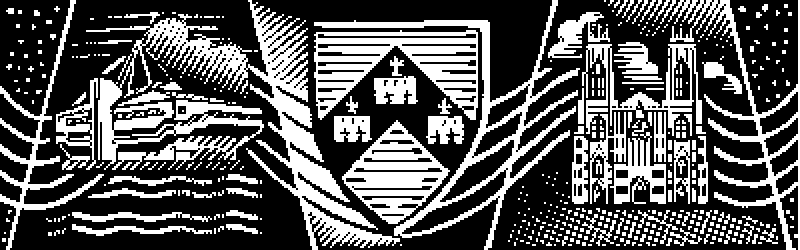
\includegraphics [width=7cm] {Woodcuts/univwoodcut}
%\end{center}
%\end{figure}
}

\newpage
\newpage
\newpage

\pagenumbering{arabic}

% (1.1) to whom: it goes to the second page immediately after the title page
\dedication{I feel it a great honour to dedicate my PhD thesis to my beloved parents for their significant contribution in achieving the goal of academic excellence reflected in my dissertation.
}

%%inroduction
\ychapter{Introduction and Motivation}{Introduction and
Motivation}{In this chapter we give a brief introduction and motivation for the research work presented in this thesis. We commence by introducing the problems in random testing. We then describe the alternative approaches to overcome these problems, followed by our research goals and contributions. At the end of the chapter, we give an outline of the thesis.

\section{The Problems}
In software testing, one is often confronted with the problem of selecting a test data set because exhaustive testing is not always applicable. Manual test data generation is a time-consuming and laborious exercise, therefore, automated test data generation is always preferred. Test data set is a subset of domain carefully selected to test the given software. Finding an adequate test data set is a crucial process in any testing technique as it aims to represent the whole infinite domain and evaluate the given system under test (SUT) for structural or functional properties \cite{mccabe1983} \cite{howden1986}. Test data generators are classified in to Pathwise, Goal-Oriented, Intellighent and Random \cite{wiki2013}. Random test data generation generate test data set randomly from the whole domain. Unlike other approaches Random approach is simple, easy to implement, fastest in computation and free from bias \cite{Ciupa2007}. \\ 
Despite the benefits random testing offers, its simplistic and non-systematic nature expose it to high criticism. \cite{Myers2004} mentioned it as "Probably the poorest methodology of all is random-input testing...". Where this statement is based on intuit n instead of experimental results but even if it is considered correct it is worth while to upgrade the strategy to generate more fault revealing test data. Random testing is also considered notorious for providing low code coverage \cite{Offutt1996}. For example, in random testing when the statement  ``if (x == 25) then ... "  is exposed to execution then there is only one chance, of the ``then..." part of the statement, to be executed out of $2^\text{32}$. If x is an integer variable of 32 bit value \cite{Godefroid2005}. Random testing is no exception when it comes to evaluate the results. Modern testing techniques deal with it by truncating the lengthy log files and display only the fault revealing test cases in the form of unit tests. However effort is required to show the test results in more compact and user friendly way. 


\section{Our Goals}
The overall goal of this thesis is to develop new techniques for automated testing based on random strategy that addresses the above mentioned problems. Particularly,

\begin{enumerate}
\item We aim to develop an automated testing technique which is able to generate more fault revealing test data out of the whole domain. In particular, it takes benefit of the presence of fault clusters found in the form of block and strip fault domains in the whole domain. Hence, we can automatically generate more fault revealing test data to evaluate the given SUT. Thus we are able to handle the problem of generating arbitrary data by random testing. 

\item We aim to develop a novel framework for finding the faults, their domains and their presentation on a graphical chart inside the specified lower and upper bound. It
considers the correlations of the fault and fault domain. It also gives a simplified and user friendly report to easily identify the faulty regions across the whole domain.

\item We aim to develop an automated strategy that utilises the literals of the SUT to particularly increase the total coverage and ultimately the overall results. On test initialisation it scan binary of the given SUT for literals. These literals are added to the prioritised list of interesting values to increase coverage and test performance. Thus we are able to handle the problem of coverage by random testing. 
\end{enumerate}

\section{Contributions}
To achieve the research goals described in Section xx, we make the following specific contributions:

\subsection{Dirt Spot Sweeping Random Strategy}
Development of a new, enhanced and improved form of automated random testing: the Dirt Spot Sweeping Random (DSSR) strategy. This strategy is based on the assumption that faults and unique failures reside in contiguous blocks and stripes. The DSSR strategy starts as a regular random+ testing strategy � a random testing technique with preference for boundary values. When a failure is found, it increases the chances of using neighbouring values of the failure in subsequent tests, thus slowly sweeping values around the failures found in hope of finding failures of different kind in its vicinity.
The DSSR strategy is implemented in the YETI random testing tool. It is evaluated against random (R) and random+ (R+) strategies by testing 60 classes (35,785 line of code) with one million (105) calls for each session, 30 times for each strategy. The results indicate that for 31 classes, all three strategies find the same unique failures. We analysed the 29 remaining classes using t-tests and found that for 7 classes DSSR is significantly better than both R+ and R, for 8 classes it performs similarly to R+ and is significantly better than R, and for 2 classes it performs similarly to ran- dom and is better than R+. In all other cases, DSSR, R+ and R do not perform significantly differently. Numerically, the DSSR strategy finds 43 more unique failures than R and 12 more unique failures than R+.

\subsection{Automated Discovery of Failure Domain}
There are several automated random strategies of software testing based on the presence of point, block and strip fault domains inside the whole input domain. As yet no particular, fully automated test strategy has been developed for the discovery and evaluation of the fault domains. We therefore have developed Automated Discovery of Failure Domain, a new random test strategy that finds the faults and the fault domains in a given system under test. It further provides visualisation of the identified pass and fail domain. In this paper we describe ADFD strategy, its implementation in YETI and illustrate its working with the help of an example. We report on experiments in which we tested error seeded one and two-dimensional numerical programs. Our experimental results show that for each SUT, ADFD strategy successfully performs identification of faults, fault domains and their representation on graphical chart.

\subsection{Random Plus Plus Strategy}
Acknowledgement of random testing being simple in implementation, quick in test case generation and free from any bias, motivated research community to do more for increase in performance, particularly, in code coverage and fault-finding ability. One such effort is Random+ --- Ordinary random testing technique with addition of interesting values (border values) of high preference. We took a step further in the same direction and developed Random++ strategy. Random++ strategy is an extended form of Random+ strategy with addition of program literals.  Literals from the given software under test are collected by instrumentation prior to testing and added to the list of interesting values.  Experimental result shows that Random++ not only increase the code coverage but also find some subtle errors that pure Random and Random+ were either unable or may take a long time to find.  



 
\section{Thesis Outline}

The rest of the thesis is organised as follows: In Chapter 2, we give a thorough review of the relevant literature. We commence by discussing a brief introduction of software testing and shed light on various techniques and types of software testing. Then, we extend our attention to automated random testing and the testing tools using random technique to test softwares. In Chapter 3, we present our first automated random strategy Dirt Spot Sweeping Random (DSSR) strategy based on sweeping faults from the clusters in the input domain. Chapter 4 describes our second automated random strategy which focus on dynamically finding the fault with their domains and its graphical representation. Chapter 5 presents the third strategy that focus on quick identification of faults and increase in coverage with the help of literals; Finally, in Chapter 7, we summarise the contributions of this thesis, discuss the weaknesses in the work, and suggest avenues for future work.






%Today, the primary focus of software companies is to achieve high quality. These companies spend an estimated thirty to ninety percent of the total software development cost on testing \ref{Beizer1990}, \ref{Standards2002}. In spite of spending 

%Software testing is the process of executing a software with specific test data followed by evaluation of the results to check whether it is working according to its specification or not \ref{Sommerville2006}.
% check here if we can replace specification with oracle or not.
%The test passes if the output complies to its specification and fails otherwise. The success of testing correlates with the number of failures found in the Software Under Test (SUT): a test is more successful if it finds more faults.

%It is interesting that program testing is used to show the presence of bugs, rather than absence of bugs [6]. Therefore the SUT that passes all the tests without returning a single failure does not guarantee that there is no fault. The testing process increases however the reliability and confidence of both the developers and the users in the tested product [7] [8] [9].

%Random testing is a black-box testing technique in which the SUT is executed against ran- domly selected test data. Test results obtained are compared either against the oracle defined, using SUT specifications in the form of assertions or exceptions defined by the programming language. The rapid increase in software development in today?s modern world prompts the need for automated testing to ensure high quality. The generation of random test data is com- paratively cheap and does not require too much intellectual and computation efforts [10] [11]. It is for this reason that various researchers have recommended this strategy for incorporation in automatic testing tools [12]. YETI [13] [14], AutoTest [15] [16], QuickCheck [17], Randoop [18], JArtage [19] are a few of the most common tools based on random strategy.
}


%%literature review
\ychapter{Literature Review}{Literature
Review\label{CHAP:FIELDREV}}{
\section{Software Testing}
\subsection{Categories of Software Testing}
\subsubsection{Black-box Testing}
\subsubsection{White-box Testing}
\subsection{Manual Testing}
\subsection{Automated Testing}
\subsubsection{Random Testing}
\subsubsection{Exhaustive Testing}

\section{Automated Random Testing}
\subsection{Test Data Generation}
\subsection{Test Execution}
\subsection{Test Oracle}
\subsection{Test Report}

\section{Variations is Random Testing}
\subsection{Adaptive Random Testing}
\subsection{Mirror Adaptive Random Testing}
\subsection{Directed Automated Random Testing}
\subsection{Quasi Random Testing}
\subsection{Monti Carlo Random Testing}
\subsection{Good Random Testing}
\subsection{Feedback-directed Random Testing}
\subsection{Adaptive Random Testing for Object-Oriented}
\subsection{Restricted Random Testing}

\section{Automated Random Testing Tools}
\subsection{JCrasher}
\subsection{JArtage}
\subsection{Eclat}
\subsection{JTest}
\subsection{QuickCheck}
\subsection{AgitarOne}
\subsection{Autotost}
\subsection{TestEra}
\subsection{Korat}
\subsection{RANDOOP}
\subsection{YETI}


\section{Conclusion}


}%{\input{FieldReview}}

%% The chapter on plan-based reward shaping.
%\ychapter{Design OR Title of the Paper}{Design OR Title of the
%Paper\label{CHAP:STRIPS}}{\input{STRIPS_Rshaping}}

%% The chapter on r-s from mixed resolution function approximation
\ychapter{Extraction of Multilingual Lexicons from
Wikipedia}{Extraction of Multilingual Lexicons from
Wikipedia\label{CHAP:DOUBLECMAC}}{\input{MultilingualLexiconsFromWikipedia}}%{\input{TwoAbstractionsInCMAC}}

%% The chapter on the Reward Shaping Analysis in model-free RL
%\ychapter{Extraction of Multilingual Synsets from Aligned
%Corpora}{Extraction of Multilingual Synsets from Aligned
%Corpora\label{CHAP:RSANALYSIS}}{\input{Rshaping_Analysis}}

\ychapter{Extraction of Multilingual Synsets from Aligned
Corpora}{Extraction of Multilingual Synsets from Aligned
Corpora\label{CHAP:MULTSYNSETS}}{\input{MultilingualSynsets}}

\ychapter{Morphology and Lexical Distances}{Morphology and Lexical
Distances\label{CHAP:MORPHLEX}}{\input{MorphologyLexicalDistances}}

%% The chapter on the use of knowledge-based admissible models in PAC-MDP learning
%\ychapter{Evaluation on Artificial Corpus}{Evaluation on Artificial
%Corpus\label{CHAP:PACMDPADMISSMODELS}}{\input{PACMDP_Admissible_Models}}

%% The chapter on the Analysis of Eligibility Traces
%\ychapter{Analysis of Exploration with Eligibility Traces}{Analysis of Exploration with Eligibility Traces\label{CHAP:ELTRACES}}{\input{Eligibility_Traces_Analysis}}

%%conclusion
\ychapter{Conclusion}{Conclusion\label{CHAP:CONCLUSION}}{\section{Conclusion}

The main goal of the present study was to develop a new random strategy which could find more faults in lower number of test cases and shorter execution time. The experimental findings revealed that DSSR strategy was up to 30\% more effective in finding faults as compared to random test strategy. The DSSR strategy not only gave more consistent results but it proved more effective in terms of detecting faults as compared to random testing. However in comparison to random plus strategy both perform equally well in 95% of the experiments but in 5% random plus perform better and faster then DSSR strategy which is due to the fact that programs contain errors in the form of point patterns and adding fault neighbouring values only increases processing without improving results. \\

Improvement in performance of DSSR strategy over random strategy was achieved by taking advantage of Random Plus and fault neighbouring values. Random plus incorporated not only border values but it also added values having higher chances of finding faults in the SUT to the list of interesting values.\\

The DSSR strategy is highly effective in case of systems containing block and strip pattern of failure across the input domain.\\

Due to the additional steps of scanning the list of interesting values for better test values and addition of fault finding test value and its neighbour values, the DSSR strategy takes upto 5\% more time to execute equal number of test cases than pure random testing and 3% more than random plus. \\

In the current version of DSSR strategy, it might depend on random or random plus strategy for finding the first fault if the fault test value was not in the list of interesting values. Once the first fault is found only then DSSR strategy could make an impact on the performance of test strategy.\\

The limitation of random plus strategy is that it maintains a static list of interesting values which remains the same for each program under test, and can be effective in many cases but not always. The better approach will be to have a dynamic list of interesting values that is automatically updated for every program which can be achieved by adding the program literals and its surrounding values to the list of interesting values prior to starting every new test session.




}


% %%%%%%%%%%%%%%%%%%%%% APPENDIX ETC %%%%%%%%%%%%%%%%%%%%%%%%%%%%%%%%%%%%

%\begin{appendix}
%\addcontentsline{toc}{chapter}{Appendices}
%--  \input{desertquestionnaire}
%--  \input{restoquestionnaire}
%--  \input{desertgraph}
%\end{appendix}


% (*) Definitions before glossary. Definitions can be easily done with the nomencl package (used in the thesis template from Cambridge).

% (*) Glossary before references.
% %  \input{}
% %   \yorkGlossary  Terms that require explanation
% %                     shall be defined in a glossary, which shall
% %                     include a key to any abbreviations used. For
% %                     an abbreviation not in common use, the term
% %                     shall be given in full at the first instance
% %                     followed by the abbreviation in brackets.
%   \input{Cglossary}

%\backmatter
%bibtex setup and path names

%latex get crazy if we don't disconnect natbib citeindex
\citeindexfalse
\renewcommand{\bibname}{References}
\bibliographystyle{newapa}
%\bibliography{../../mybib}
\bibliography{mybib}

%\yorkBib{}


% index.bat has to be executed to process index files.
\yorkIndex
\yorkCiteIndex
\yorkNomIndex

\begin{figure}[b]
 \begin{center}
 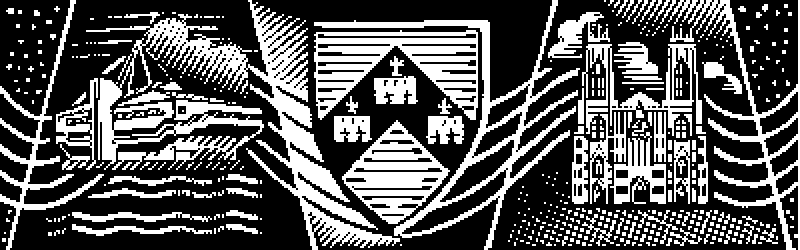
\includegraphics [width=7cm] {Woodcuts/univwoodcut}
\end{center}
\end{figure}

%\ylastpage{
%\begin{picture}(0.0,0.0)
%  \put(80,-550){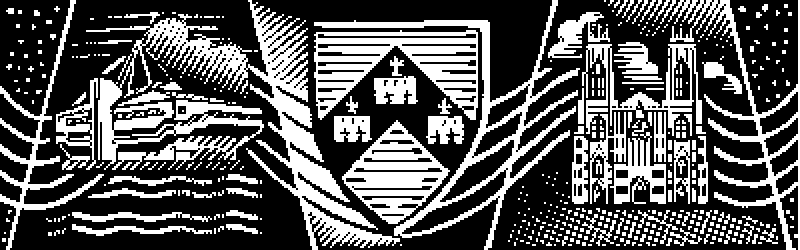
\includegraphics[width=7cm]{Woodcuts/univwoodcut}}
%\end{picture}
%}


%\listoftodos




\end{document}
